\documentclass[]{beamer}
% Class options include: notes, notesonly, handout, trans,
%                        hidesubsections, shadesubsections,
%                        inrow, blue, red, grey, brown

% Theme for beamer presentation.
\usepackage{beamerthemesplit} 
% Other themes include: beamerthemebars, beamerthemelined, 
%                       beamerthemetree, beamerthemetreebars  

\title{A Network-based Analysis of Technology-driven and Load-driven Constraints in Production Data}
\author{Serhat Kosif}
\institute{Jacobs University}
\date{Spring Semester 2021}

\begin{document}
	
	\begin{frame}[plain]
		\titlepage
	\end{frame}
	\note{Talk for 30 minutes} % Add notes to yourself that will be displayed when
	% typeset with the notes or notesonly class options
	
	\section[Outline]{}
	
	% Creates table of contents slide incorporating
	% all \section and \subsection commands
	\begin{frame}
		\tableofcontents
	\end{frame}
	
	
	\section{Feature Projection on Different Networks}
	
	\begin{frame}
		\frametitle{Features to be Projected}   
		\begin{columns}[c]
			\column{2in}  % slides are 3in high by 5in wide
			Steel Grade Network with Single Data Points
			\framebox{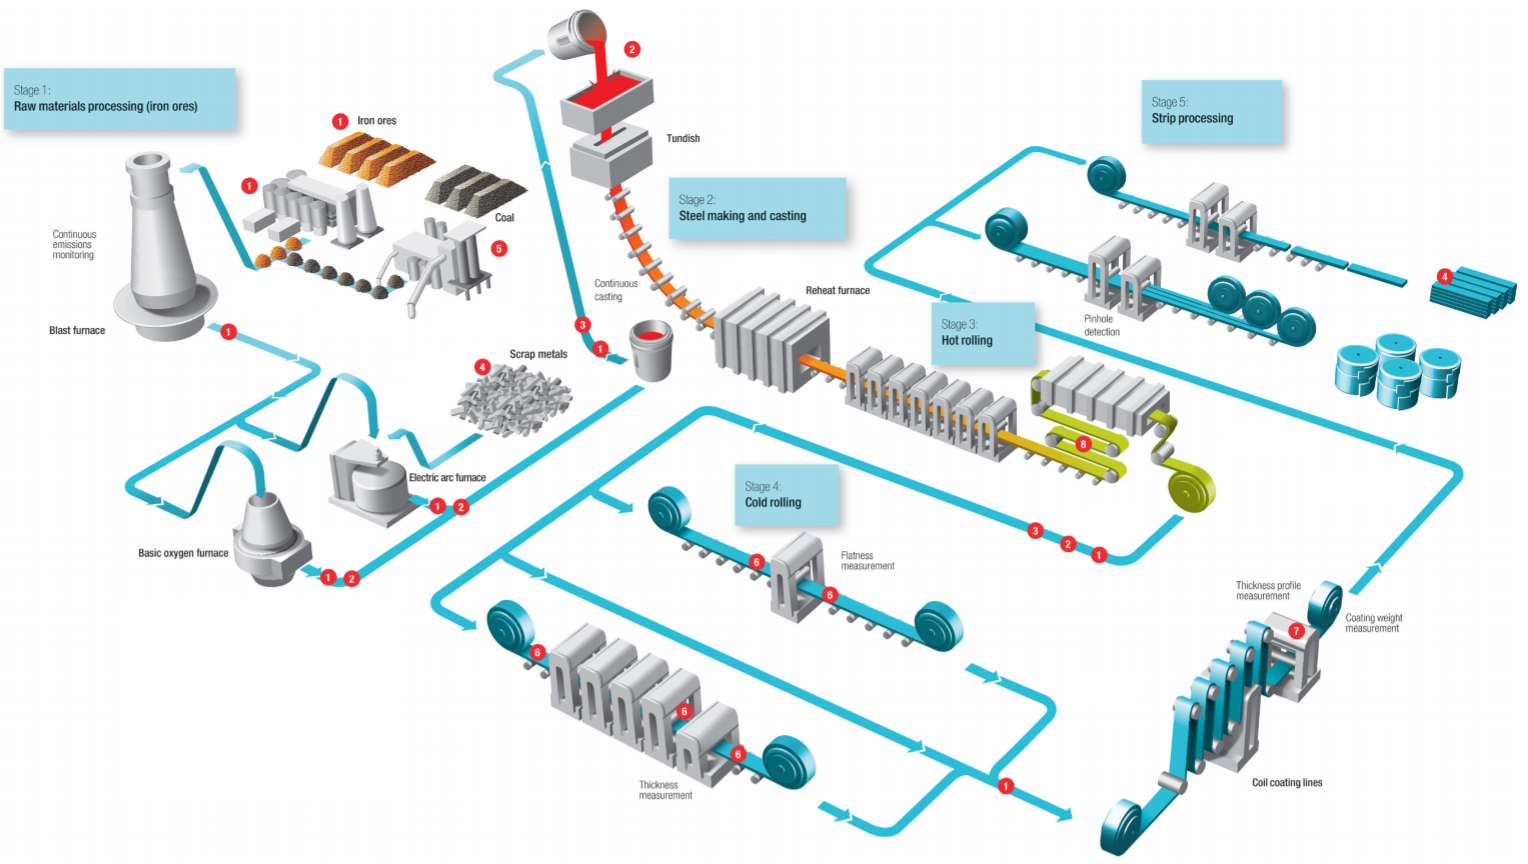
\includegraphics[height=1.8in]{../images/steel-production-steps.png}}
			\column{2in}
			Width Network with Constant Data Intervals
			\framebox{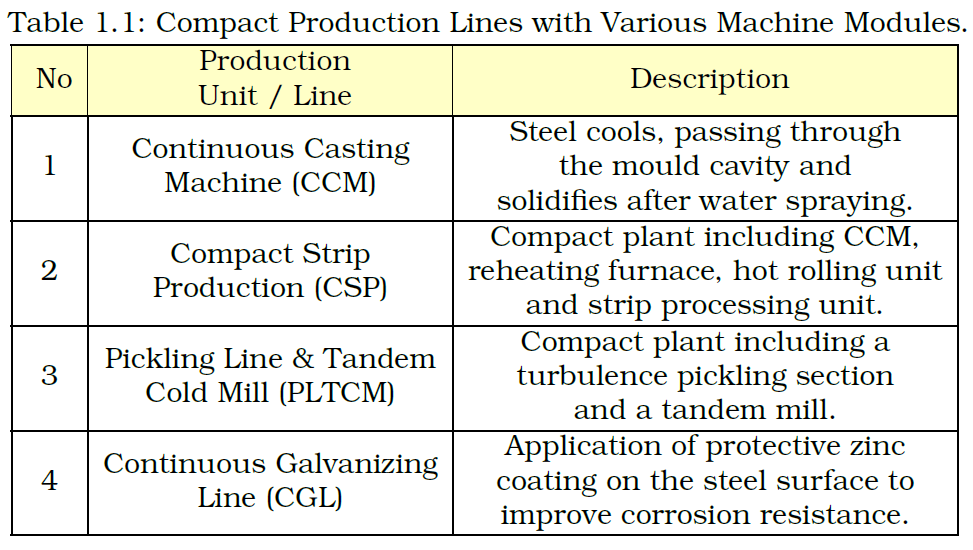
\includegraphics[height=1.8in]{../tables/production_lines.png}}
		\end{columns}
	\end{frame}
	%\note[enumerate]       % Add notes to yourself that will be displayed when
	%{                      % typeset with the notes or notesonly class options
	%\item Steel Grade Projections   
	%\item Width Projections   
	%}
	
	
	
	\note{The end}       % Add notes to yourself that will be displayed when
	% typeset with the notes or notesonly class options
	
\end{document}
